% ==============================================================================
% Results
% ==============================================================================

\section{Results}
\label{sec:results}

% -------------------------------------------------------------------
\subsection{Behavioral Validation}
\label{sec:results_behavioral}

\textbf{[Result placeholder.]}  Table~\ref{tab:behavioral} reports model
accuracy and S1-lure rates across all seven task categories.

\begin{table}[t]
\centering
\caption{Behavioral results: accuracy (\%) and S1-lure rate (\%) on conflict
  and no-conflict items.  Standard models are expected to show higher lure
  rates on conflict items; reasoning models should partially overcome this
  pattern.}
\label{tab:behavioral}
\vspace{4pt}
\small
\begin{tabular}{lcccc}
\toprule
& \multicolumn{2}{c}{\textbf{Conflict}} & \multicolumn{2}{c}{\textbf{No-Conflict}} \\
\cmidrule(lr){2-3}\cmidrule(lr){4-5}
\textbf{Model} & Acc. & Lure \% & Acc. & Lure \% \\
\midrule
Llama-3.1-8B-Instruct   & -- & -- & -- & -- \\
Gemma-2-9B-IT            & -- & -- & -- & -- \\
R1-Distill-Llama-8B     & -- & -- & -- & -- \\
R1-Distill-Qwen-7B      & -- & -- & -- & -- \\
\bottomrule
\end{tabular}
\end{table}

% -------------------------------------------------------------------
\subsection{Linear Probes}
\label{sec:results_probes}

\textbf{[Result placeholder.]}  Figure~\ref{fig:probe_accuracy} shows
layer-wise probe ROC-AUC for the conflict/no-conflict classification target
across all four models.

\begin{figure}[t]
\centering
% \includegraphics[width=\linewidth]{figures/fig2_probe_accuracy.pdf}
\fbox{\parbox{0.95\linewidth}{\centering\vspace{2cm}
  \textbf{Figure 2: Layer-wise probe accuracy}\\[4pt]
  \small X-axis: layer index.  Y-axis: ROC-AUC.\\
  4 model curves with bootstrap 95\% CIs.\\
  Dashed line: Hewitt--Liang control task performance.\\
  Gray band: permutation test 95th percentile.
\vspace{2cm}}}
\caption{Layer-wise probe ROC-AUC for classifying conflict versus
  no-conflict items from residual stream activations at position~P0.
  Shaded bands show bootstrap 95\% CIs.  The dashed line indicates
  Hewitt--Liang control task performance (selectivity floor).  [We find
  that \ldots]}
\label{fig:probe_accuracy}
\end{figure}

\paragraph{Selectivity.}  [Report selectivity = real accuracy $-$ control
accuracy at the peak layer for each model.  Only selectivity $>$ 5pp is
meaningful.]

\paragraph{Cross-category generalization.}  [Report leave-one-category-out
accuracy.  If it holds, the probe learned a domain-general signal.]

\paragraph{Nonlinearity check.}  [Compare logistic regression vs.\ MLP probe
accuracy.  If MLP substantially outperforms, the signal has a nonlinear
component.]

% -------------------------------------------------------------------
\subsection{SAE Feature Analysis}
\label{sec:results_sae}

\textbf{[Result placeholder.]}  Figure~\ref{fig:volcano} shows the volcano
plot of differential SAE feature activation.

\begin{figure}[t]
\centering
% \includegraphics[width=\linewidth]{figures/fig3_sae_volcano.pdf}
\fbox{\parbox{0.95\linewidth}{\centering\vspace{2cm}
  \textbf{Figure 3: SAE volcano plot}\\[4pt]
  \small X-axis: log fold-change (conflict vs.\ no-conflict).\\
  Y-axis: $-\log_{10}(p)$ (BH-FDR corrected).\\
  Upper-left: ``heuristic features.''\\
  Upper-right: ``deliberation features.''\\
  Red points: features surviving Ma et al.\ falsification.\\
  Gray points: features failing falsification.
\vspace{2cm}}}
\caption{Volcano plot of SAE feature activation differences between
  conflict and no-conflict items (Llama-3.1-8B-Instruct, layer~[X]).
  Features in the upper corners show large, statistically significant
  differential activation.  Red: features surviving falsification
  \citep{ma2026falsification}; gray: spurious features eliminated by the
  falsification protocol.  [We identify \ldots]}
\label{fig:volcano}
\end{figure}

\paragraph{Falsification rates.}  [Report: of $N$ candidate features, $M$
($X$\%) survived the Ma et al.\ falsification protocol.  Compare to Ma et
al.'s reported 45--90\% spurious rate.]

\paragraph{Feature interpretation.}  [For the top-$K$ surviving features,
report (i)~top activating examples, (ii)~decoder direction cosine similarity
to known features, (iii)~activation patterns across task categories.]

% -------------------------------------------------------------------
\subsection{Causal Interventions}
\label{sec:results_causal}

\textbf{[Result placeholder.]}  Figure~\ref{fig:causal} shows the effect
of amplifying and ablating candidate deliberation features on model behavior.

\begin{figure}[t]
\centering
% \includegraphics[width=\linewidth]{figures/fig4_causal_bars.pdf}
\fbox{\parbox{0.95\linewidth}{\centering\vspace{2cm}
  \textbf{Figure 4: Causal intervention results}\\[4pt]
  \small Grouped bar chart.\\
  Groups: Amplify S2 features / Ablate S2 features / Random direction.\\
  Bars: $\Delta$ P(correct) and $\Delta$ P(lure).\\
  Error bars: $\pm$ 1 SE across 3 seeds.
\vspace{2cm}}}
\caption{Causal intervention results.  Amplifying candidate deliberation
  features [increases/does not change] $P(\text{correct})$ on conflict
  items, while ablating them [increases/does not change]
  $P(\text{S1-lure})$.  Steering along a random direction of the same norm
  produces negligible change ($\Delta < [X]$).}
\label{fig:causal}
\end{figure}

\paragraph{Dose-response.}  [Report: $\Delta P(\text{correct})$ as a
function of steering coefficient $\alpha$.  Expected: monotonic increase
to a plateau, then degradation at extreme values.]

\paragraph{Side effects.}  [Report: change in general capability on a
held-out task set.  Steering should not degrade non-bias performance.]

% -------------------------------------------------------------------
\subsection{Attention Entropy}
\label{sec:results_attention}

\textbf{[Result placeholder.]}  Figure~\ref{fig:entropy} shows the
distribution of per-head attention entropy on conflict versus no-conflict
items.

\begin{figure}[t]
\centering
% 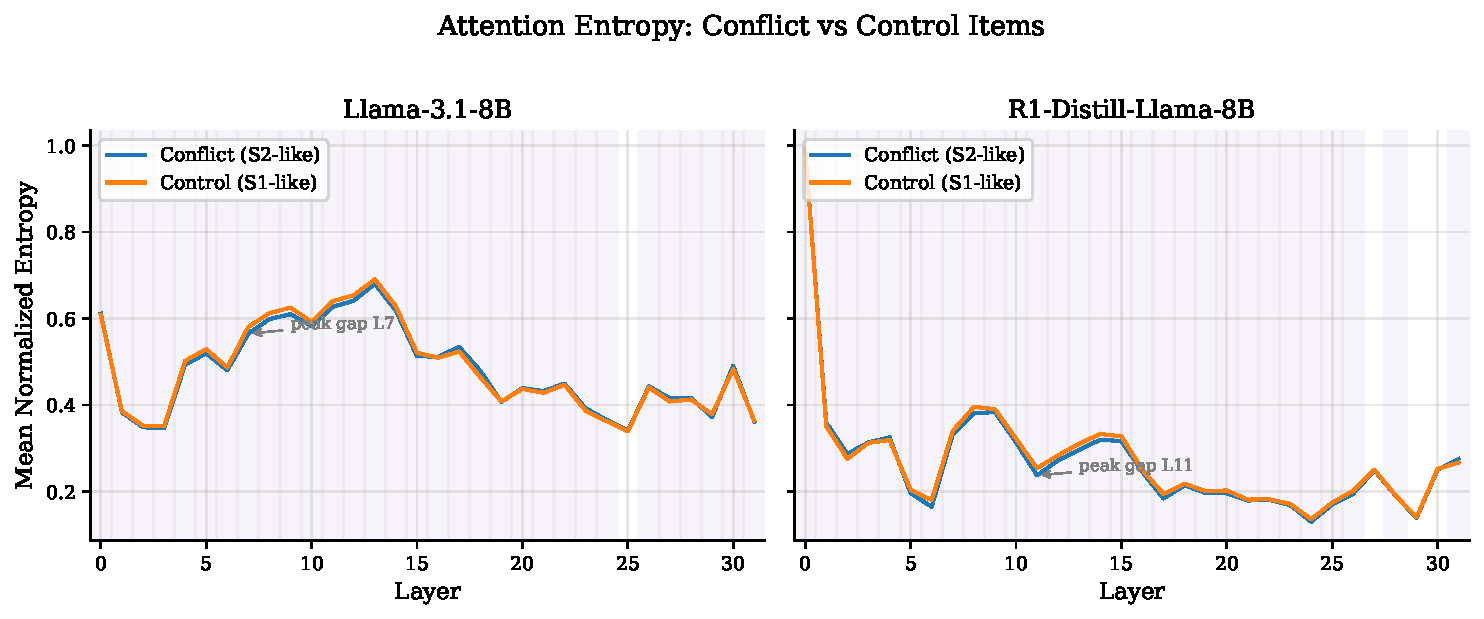
\includegraphics[width=\linewidth]{figures/fig5_attention_entropy.pdf}
\fbox{\parbox{0.95\linewidth}{\centering\vspace{2cm}
  \textbf{Figure 5: Attention entropy ridge plots}\\[4pt]
  \small Y-axis: layer groups (early / mid / late).\\
  X-axis: normalized attention entropy.\\
  Blue: conflict items.  Orange: no-conflict items.\\
  One panel per model.
\vspace{2cm}}}
\caption{Distribution of normalized attention entropy on conflict (blue) and
  no-conflict (orange) items, grouped by layer position.  [We find that
  \ldots]}
\label{fig:entropy}
\end{figure}

\paragraph{Head classification.}  [Report: proportion of heads classified as
S2-specialized, S1-specialized, or unspecialized for each model.  Compare
at query-head and KV-group granularity.]

\paragraph{Temporal dynamics.}  [For reasoning models: compare entropy
trajectories within the thinking trace on conflict vs.\ no-conflict items.]

% -------------------------------------------------------------------
\subsection{Representational Geometry}
\label{sec:results_geometry}

\textbf{[Result placeholder.]}  Figure~\ref{fig:geometry} shows the
layer-wise cosine silhouette score and PCA visualizations.

\begin{figure}[t]
\centering
% \includegraphics[width=\linewidth]{figures/fig6_geometry.pdf}
\fbox{\parbox{0.95\linewidth}{\centering\vspace{2cm}
  \textbf{Figure 6: Representational geometry}\\[4pt]
  \small Left: layer-wise cosine silhouette score (4 models).\\
  Right: PCA visualization at peak-separation layer.\\
  Permutation baseline shown as dashed line.
\vspace{2cm}}}
\caption{Left: layer-wise cosine silhouette score for conflict vs.\
  no-conflict activation clusters (after PCA to 50 dimensions), with
  permutation baseline (dashed).  Right: first two principal components
  at the layer of maximum separation for Llama-3.1-8B-Instruct.  [We find
  that \ldots]}
\label{fig:geometry}
\end{figure}

\paragraph{CKA.}  [Report: layer-matched CKA between Llama-3.1-8B-Instruct
and R1-Distill-Llama-8B, separately for conflict and no-conflict items.]

\paragraph{Intrinsic dimensionality.}  [Report: Two-NN estimates for S1-like
vs.\ S2-like activation clouds at the peak-separation layer.]

% -------------------------------------------------------------------
\subsection{Cross-Workstream Convergence}
\label{sec:results_convergence}

\textbf{[Result placeholder.]}  [Synthesize: which layers show consistent
S1/S2 signals across probes, SAE features, attention entropy, and geometry?
Do the methods agree on which layers and positions carry the most
deliberation-intensity information?  Do they agree across models?]
